% AUTO-GENERATED by code/figlib.py helpers -- do not edit
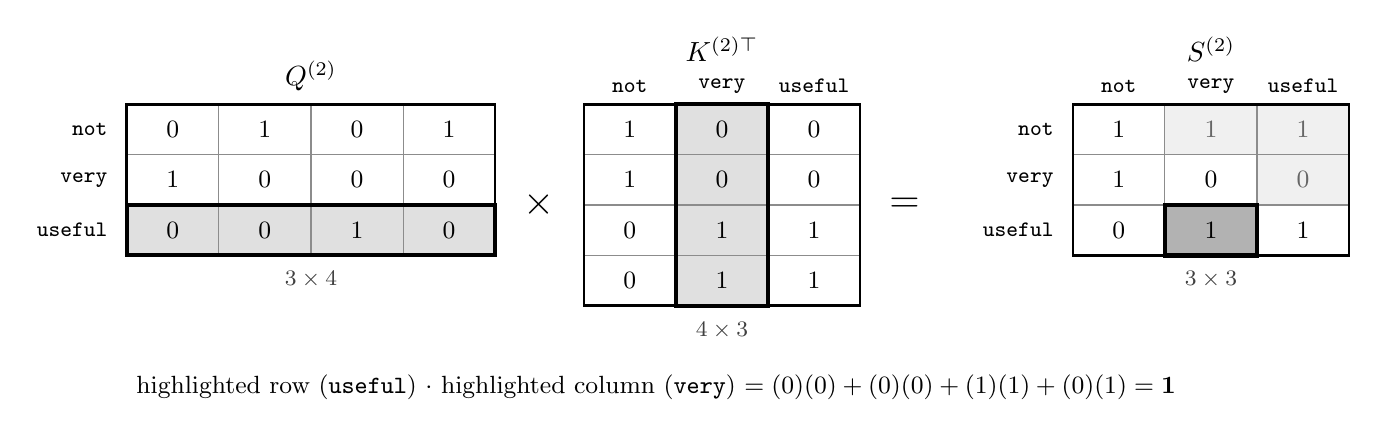
\begin{tikzpicture}[x=1.5cm]
\draw[black!45, fill=white] (0.000,0.000) rectangle (0.780,-0.640);
\node[font=\small, text=black] at (0.390,-0.320) {$0$};
\draw[black!45, fill=white] (0.780,0.000) rectangle (1.560,-0.640);
\node[font=\small, text=black] at (1.170,-0.320) {$1$};
\draw[black!45, fill=white] (1.560,0.000) rectangle (2.340,-0.640);
\node[font=\small, text=black] at (1.950,-0.320) {$0$};
\draw[black!45, fill=white] (2.340,0.000) rectangle (3.120,-0.640);
\node[font=\small, text=black] at (2.730,-0.320) {$1$};
\draw[black!45, fill=white] (0.000,-0.640) rectangle (0.780,-1.279);
\node[font=\small, text=black] at (0.390,-0.959) {$1$};
\draw[black!45, fill=white] (0.780,-0.640) rectangle (1.560,-1.279);
\node[font=\small, text=black] at (1.170,-0.959) {$0$};
\draw[black!45, fill=white] (1.560,-0.640) rectangle (2.340,-1.279);
\node[font=\small, text=black] at (1.950,-0.959) {$0$};
\draw[black!45, fill=white] (2.340,-0.640) rectangle (3.120,-1.279);
\node[font=\small, text=black] at (2.730,-0.959) {$0$};
\draw[black!45, fill=black!12] (0.000,-1.279) rectangle (0.780,-1.919);
\node[font=\small, text=black] at (0.390,-1.599) {$0$};
\draw[black!45, fill=black!12] (0.780,-1.279) rectangle (1.560,-1.919);
\node[font=\small, text=black] at (1.170,-1.599) {$0$};
\draw[black!45, fill=black!12] (1.560,-1.279) rectangle (2.340,-1.919);
\node[font=\small, text=black] at (1.950,-1.599) {$1$};
\draw[black!45, fill=black!12] (2.340,-1.279) rectangle (3.120,-1.919);
\node[font=\small, text=black] at (2.730,-1.599) {$0$};
\draw[line width=1.4pt] (0.000,-1.279) rectangle (3.120,-1.919);
\draw[line width=0.9pt] (0.000,0.000) rectangle (3.120,-1.919);
\node[anchor=east, font=\footnotesize\ttfamily] at (-0.080,-0.320) {not};
\node[anchor=east, font=\footnotesize\ttfamily] at (-0.080,-0.959) {very};
\node[anchor=east, font=\footnotesize\ttfamily] at (-0.080,-1.599) {useful};
\node[anchor=south, font=\normalsize] at (1.560,0.050) {$Q^{(2)}$};
\node[anchor=north, font=\footnotesize, text=black!75] at (1.560,-1.999) {$3\times4$};
\draw[black!45, fill=white] (3.870,0.000) rectangle (4.650,-0.640);
\node[font=\small, text=black] at (4.260,-0.320) {$1$};
\draw[black!45, fill=black!12] (4.650,0.000) rectangle (5.430,-0.640);
\node[font=\small, text=black] at (5.040,-0.320) {$0$};
\draw[black!45, fill=white] (5.430,0.000) rectangle (6.210,-0.640);
\node[font=\small, text=black] at (5.820,-0.320) {$0$};
\draw[black!45, fill=white] (3.870,-0.640) rectangle (4.650,-1.279);
\node[font=\small, text=black] at (4.260,-0.959) {$1$};
\draw[black!45, fill=black!12] (4.650,-0.640) rectangle (5.430,-1.279);
\node[font=\small, text=black] at (5.040,-0.959) {$0$};
\draw[black!45, fill=white] (5.430,-0.640) rectangle (6.210,-1.279);
\node[font=\small, text=black] at (5.820,-0.959) {$0$};
\draw[black!45, fill=white] (3.870,-1.279) rectangle (4.650,-1.919);
\node[font=\small, text=black] at (4.260,-1.599) {$0$};
\draw[black!45, fill=black!12] (4.650,-1.279) rectangle (5.430,-1.919);
\node[font=\small, text=black] at (5.040,-1.599) {$1$};
\draw[black!45, fill=white] (5.430,-1.279) rectangle (6.210,-1.919);
\node[font=\small, text=black] at (5.820,-1.599) {$1$};
\draw[black!45, fill=white] (3.870,-1.919) rectangle (4.650,-2.558);
\node[font=\small, text=black] at (4.260,-2.239) {$0$};
\draw[black!45, fill=black!12] (4.650,-1.919) rectangle (5.430,-2.558);
\node[font=\small, text=black] at (5.040,-2.239) {$1$};
\draw[black!45, fill=white] (5.430,-1.919) rectangle (6.210,-2.558);
\node[font=\small, text=black] at (5.820,-2.239) {$1$};
\draw[line width=1.4pt] (4.650,0.000) rectangle (5.430,-2.558);
\draw[line width=0.9pt] (3.870,0.000) rectangle (6.210,-2.558);
\node[anchor=south, font=\footnotesize\ttfamily] at (4.260,0.020) {not};
\node[anchor=south, font=\footnotesize\ttfamily] at (5.040,0.020) {very};
\node[anchor=south, font=\footnotesize\ttfamily] at (5.820,0.020) {useful};
\node[anchor=south, font=\normalsize] at (5.040,0.420) {$K^{(2)\top}$};
\node[anchor=north, font=\footnotesize, text=black!75] at (5.040,-2.638) {$4\times3$};
\draw[black!45, fill=white] (8.010,0.000) rectangle (8.790,-0.640);
\node[font=\small, text=black] at (8.400,-0.320) {$1$};
\draw[black!45, fill=black!6] (8.790,0.000) rectangle (9.570,-0.640);
\node[font=\small, text=black!60] at (9.180,-0.320) {$1$};
\draw[black!45, fill=black!6] (9.570,0.000) rectangle (10.350,-0.640);
\node[font=\small, text=black!60] at (9.960,-0.320) {$1$};
\draw[black!45, fill=white] (8.010,-0.640) rectangle (8.790,-1.279);
\node[font=\small, text=black] at (8.400,-0.959) {$1$};
\draw[black!45, fill=white] (8.790,-0.640) rectangle (9.570,-1.279);
\node[font=\small, text=black] at (9.180,-0.959) {$0$};
\draw[black!45, fill=black!6] (9.570,-0.640) rectangle (10.350,-1.279);
\node[font=\small, text=black!60] at (9.960,-0.959) {$0$};
\draw[black!45, fill=white] (8.010,-1.279) rectangle (8.790,-1.919);
\node[font=\small, text=black] at (8.400,-1.599) {$0$};
\draw[black!45, fill=black!30] (8.790,-1.279) rectangle (9.570,-1.919);
\node[font=\small, text=black] at (9.180,-1.599) {$1$};
\draw[black!45, fill=white] (9.570,-1.279) rectangle (10.350,-1.919);
\node[font=\small, text=black] at (9.960,-1.599) {$1$};
\draw[line width=1.6pt] (8.790,-1.279) rectangle (9.570,-1.919);
\draw[line width=0.9pt] (8.010,0.000) rectangle (10.350,-1.919);
\node[anchor=east, font=\footnotesize\ttfamily] at (7.930,-0.320) {not};
\node[anchor=east, font=\footnotesize\ttfamily] at (7.930,-0.959) {very};
\node[anchor=east, font=\footnotesize\ttfamily] at (7.930,-1.599) {useful};
\node[anchor=south, font=\footnotesize\ttfamily] at (8.400,0.020) {not};
\node[anchor=south, font=\footnotesize\ttfamily] at (9.180,0.020) {very};
\node[anchor=south, font=\footnotesize\ttfamily] at (9.960,0.020) {useful};
\node[anchor=south, font=\normalsize] at (9.180,0.420) {$S^{(2)}$};
\node[anchor=north, font=\footnotesize, text=black!75] at (9.180,-1.999) {$3\times3$};
\node[font=\Large] at (3.495,-1.279) {$\times$};
\node[font=\Large] at (6.585,-1.279) {$=$};
\node[anchor=north west, font=\small, align=left] at (0,-3.308) {highlighted row (\texttt{useful}) $\cdot$ highlighted column (\texttt{very}) $= (0)(0) + (0)(0) + (1)(1) + (0)(1) = \mathbf{1}$};
\end{tikzpicture}
